\subsection{Terzo sprint}

\begin{minipage}{\textwidth}
  Di seguito è riportata la distribuzione delle ore per ciascun membro del team, accumulate in totali per persona e per ruolo:
  \begin{table}[H]
    \begin{tabularx}{\textwidth}{|c|*{6}{>{\centering}X|}c|}
      \hline
      \multicolumn{8}{|c|}{\textbf{Consuntivo orario}} \\
      \hline
      \textbf{Membro del team} & \textbf{Re} & \textbf{Am} & \textbf{An} & \textbf{Pt} & \textbf{Pr} & \textbf{Ve} & \textbf{Totale per persona} \\
      \hline
      Cavalli Riccardo & 1 & 2 & 0 & 6 & 2 & 0 & 11 \\
      \hline
      Pianon Raul & 0 & 0 & 0 & 0 & 8 & 0 & 8 \\
      \hline
      Dall'Amico Martina & 0 & 8 & 0 & 0 & 0 & 0 & 8 \\ 
      \hline
      Cristo Marco & 0 & 0 & 0 & 0 & 5 & 2 & 7 \\ 
      \hline
      Lewental Sebastiano & 0 & 0 & 0 & 3 & 2 & 3 & 8 \\ 
      \hline
      Zecchinato Mattia & 0 & 1 & 5 & 0 & 0 & 0 & 6 \\ 
      \hline
      Stocco Tommaso & 4 & 0 & 0 & 0 & 0 & 2 & 6 \\ 
      \hline
      \textbf{Totale ore per ruolo} & 5 & 11 & 5 & 9 & 17 & 7 & \textbf{54} \\
      \hline
    \end{tabularx}
    \caption{Sprint 3 - Consuntivo orario}
  \end{table}
  \end{minipage}
  
  \begin{figure}[H]
    \centering
    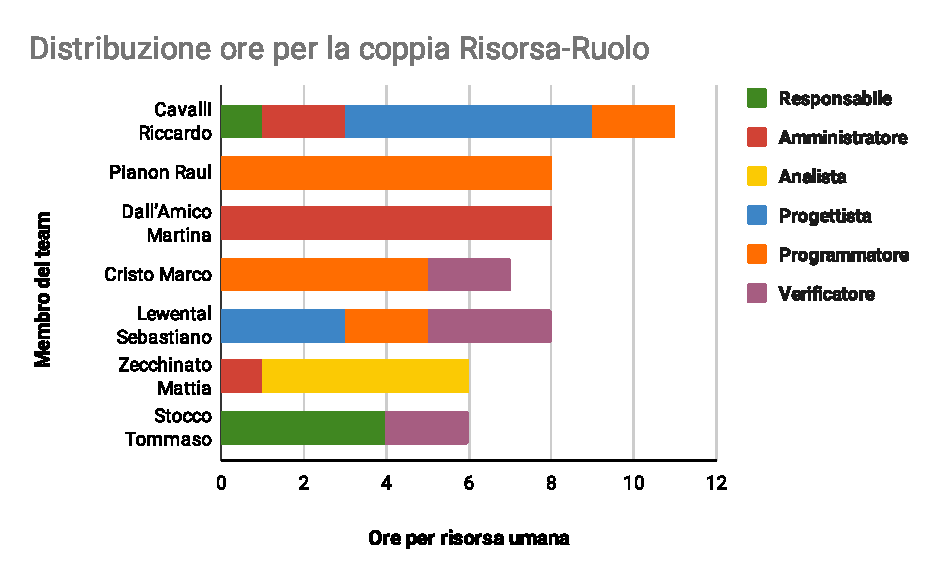
\includegraphics[width=0.90\textwidth]{assets/Consuntivo/Sprint-3/distribuzione_ore_risorsa_ruolo.pdf}
    \caption{Sprint 3 - Istogramma della distribuzione oraria per la coppia risorsa-ruolo}
  \end{figure}
  
  \begin{figure}[H]
    \centering
    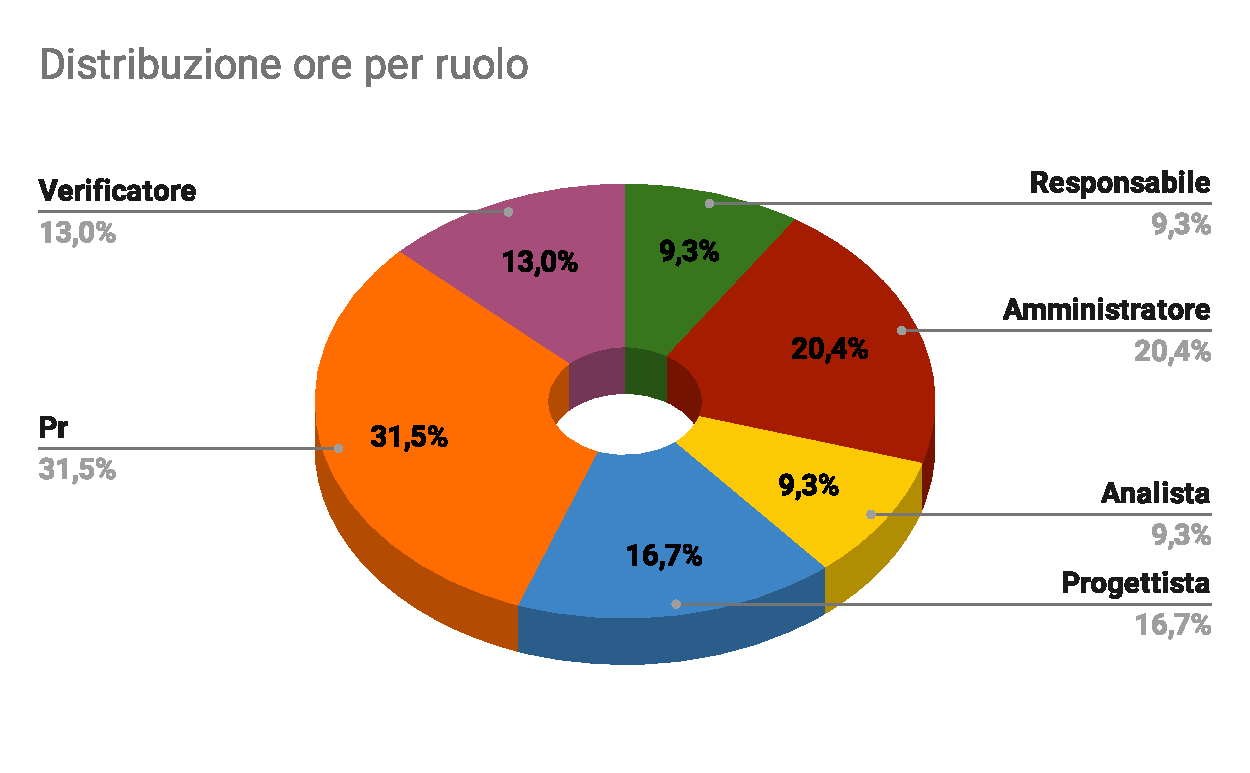
\includegraphics[width=0.90\textwidth]{assets/Consuntivo/Sprint-3/distribuzione_ore_ruolo.pdf}
    \caption{Sprint 3 - Areogramma della distribuzione oraria per ruolo}
  \end{figure}
  
  \begin{minipage}{\textwidth}
  Di seguito è riportato il consuntivo economico del terzo \glossario{sprint}:
  \begin{table}[H]
  \begin{adjustwidth}{-0.5cm}{-0.5cm}
    \centering
    \begin{tabular}{|P{2.9cm}|P{2.3cm}|P{2.5cm}|P{2.3cm}|>{\arraybackslash}P{2.5cm}|}
      \hline
      \multicolumn{5}{|c|}{\textbf{Consuntivo economico}} \\
      \hline
      \textbf{Ruolo} & \textbf{Ore per ruolo} & \textbf{Delta ore preventivo - consuntivo} & \textbf{Costo (in \texteuro)} & \textbf{Delta costo preventivo - consuntivo (in \texteuro)} \\
      \hline
      Responsabile & 5 & +1 & 150,00 & +30,00 \\ 
      \hline
      Amministratore & 11 & +1 & 220,00 & +20,00 \\ 
      \hline
      Analista & 5 & -1 & 125,00 & -25,00 \\ 
      \hline
      Progettista & 9 & -3 & 225,00 & -75,00 \\ 
      \hline
      Programmatore & 17 & -1 & 255,00 & -15,00 \\ 
      \hline
      Verificatore & 7 & 0 & 105,00 & 0,00 \\ 
      \hline
      \textbf{Totale} & \textbf{54} & -3 & \textbf{1.080,00} & -65,00 \\ 
      \hline
      \textbf{Restante} & 488 & / & 9.790,00 & / \\ 
      \hline
      \textbf{Sprint pregressi} & 95 & / & 2.150,00 & / \\ 
      \hline
    \end{tabular}
    \caption{Sprint 3 - Consuntivo economico}
  \end{adjustwidth}
  \end{table}
  \end{minipage}
  
  \begin{figure}[H]
    \centering
    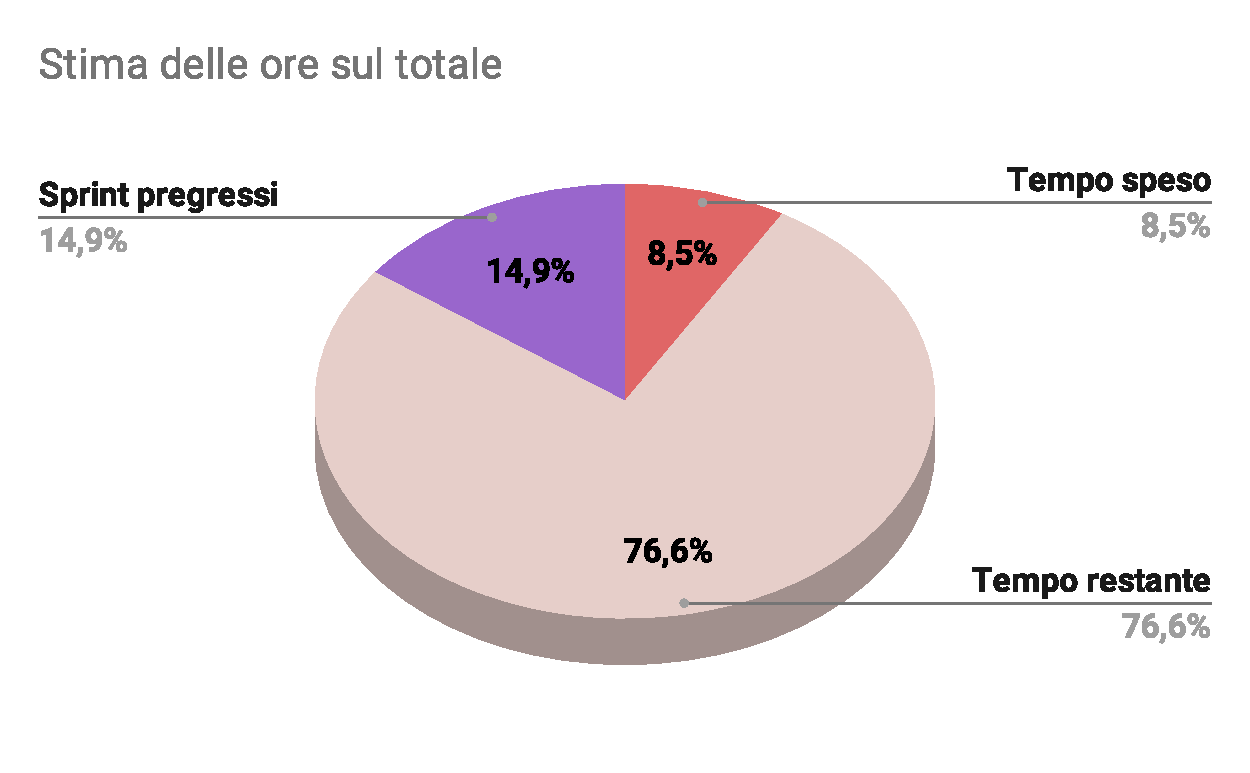
\includegraphics[width=0.90\textwidth]{assets/Consuntivo/Sprint-3/copertura_oraria.pdf}
    \caption{Sprint 3 - Areogramma del tempo speso (in ore) rispetto al totale}
  \end{figure}
  
  \begin{figure}[H]
    \centering
    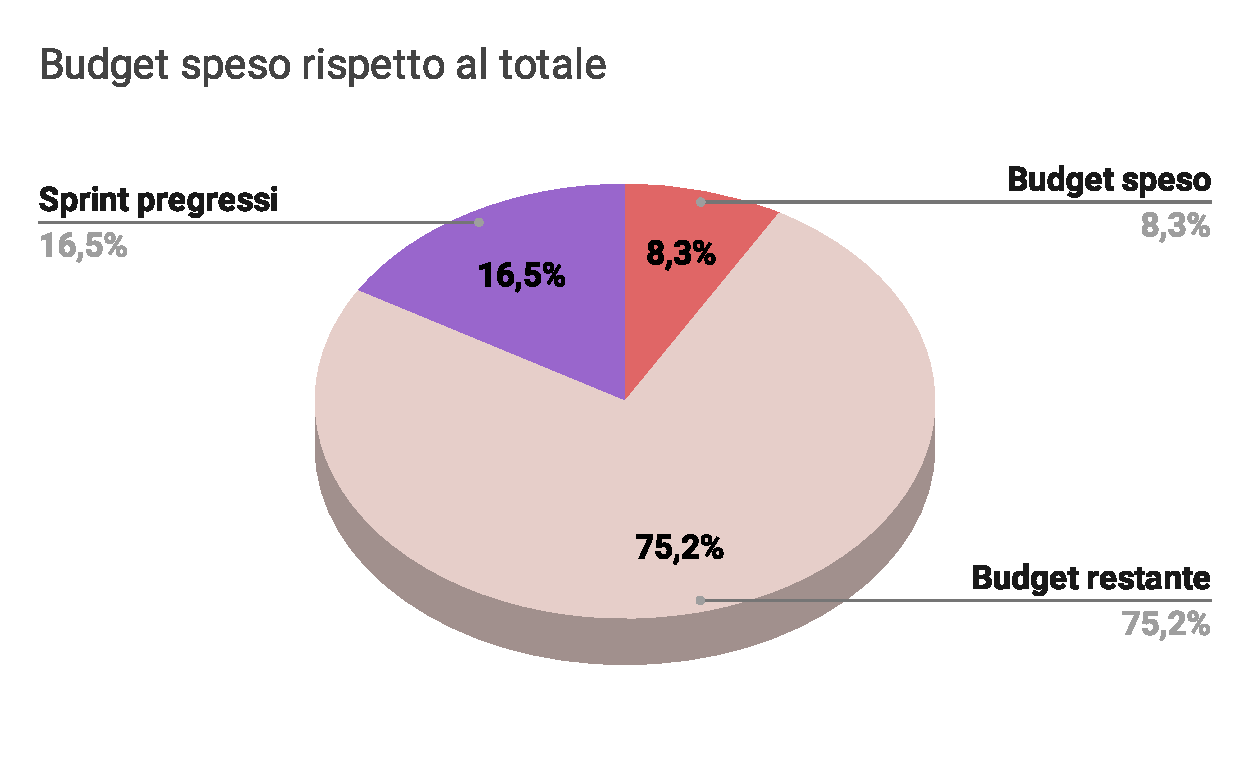
\includegraphics[width=0.90\textwidth]{assets/Consuntivo/Sprint-3/budget_speso.pdf}
    \caption{Sprint 3 - Areogramma del budget speso rispetto al totale}
  \end{figure}
  
  \begin{minipage}{\textwidth}
    Di seguito sono riportate le ore rimanenti per la coppia risorsa-ruolo:
    \begin{table}[H]
      \begin{tabularx}{\textwidth}{|c|*{6}{>{\centering}X|}c|}
        \hline
        \multicolumn{8}{|c|}{\textbf{Ore rimanenti per la coppia risorsa-ruolo}} \\
        \hline
        \textbf{Membro del team} & \textbf{Re} & \textbf{Am} & \textbf{An} & \textbf{Pt} & \textbf{Pr} & \textbf{Ve} & \textbf{Totale per persona} \\
        \hline
        Cavalli Riccardo & 0 & 0 & 9 & 17 & 20 & 20 & 66 \\ 
        \hline
        Pianon Raul & 2 & 8 & 9 & 23 & 14 & 12 & 68 \\ 
        \hline
        Dall'Amico Martina & 9 & 0 & 1 & 23 & 22 & 15 & 70 \\ 
        \hline
        Cristo Marco & 9 & 8 & 2 & 20 & 12 & 18 & 69 \\ 
        \hline
        Lewental Sebastiano & 9 & 8 & 2 & 14 & 20 & 17 & 70 \\ 
        \hline
        Zecchinato Mattia & 9 & 7 & 3 & 17 & 22 & 14 & 72 \\ 
        \hline
        Stocco Tommaso & 5 & 2 & 3 & 23 & 22 & 18 & 73 \\ 
        \hline
        \textbf{Totale ore per ruolo} & 43 & 33 & 29 & 137 & 132 & 114 & \textbf{488} \\ 
        \hline
      \end{tabularx}
      \caption{Sprint 3 - Ore rimanenti per la coppia risorsa-ruolo}
    \end{table}
  \end{minipage}

\subsubsection{Revisione delle attività}

Nell'arco del terzo \glossario{sprint}, il team ha svolto le seguenti attività:
\begin{itemize}
    \item Stesura verbali interni ed esterni;
    \item Push e pull dell'immagine \glossario{Docker} su \glossario{GitHub Container Registry};
    \item Aggiornamento delle \NdP\ con le modalità di integrazione Jira - Github;
    \item Riformulazione del dizionario dati (chiavi primarie, chiavi esterne e sinonimi);
    \item Creazione della prima bozza dell'interfaccia grafica;
    \item Studio del framework \glossario{Streamlit} e inizio sviluppo della web app;
    \item Definizione di un indice aggiuntivo per ricavare le informazioni delle tabelle pertinenti alla richiesta dell'utente;	
    \item Modifica struttura del PdP\ e approfondimento della sezione relativa al consuntivo;
    \item Selezione e descrizione delle metriche M1, M2, M3, M4;
    \item Scelta dei range di tolleranza per le metriche M1, M2, M3, M4;
    \item Benchmark iniziale dei modelli;
    \item Unificazione dei differenti metodi di estrazione del \glossario{dizionario dati} in un modulo unico;
    \item Stesura delle sezioni incomplete nel documento di \AdR\;
    \item Espansione dei casi d'uso e rifinitura delle definizioni dei requisiti e delle fonti;
    \item Approfondimento del funzionamento di \glossario{txtai};
    \item Creazione di un dizionario dati in italiano per testare il modello sentence-BERTino di efederici;
    \item Prova di traduzione della richiesta utente;
    \item Costruzione della query SQL per la ricerca semantica;
    \item Aggiunta dei sinonimi delle tabelle e delle colonne nell'\glossario{indice};
    \item Miglioramento della ricerca semantica tramite la media pesata dei punteggi;
    \item Definizione di un workflow su GitHub Actions per il repository di sviluppo;
    \item Preventivo dello sprint 4;
    \item Elaborazione di una presentazione sul framework Streamlit;
    \item Configurazione di \glossario{Flask} e \glossario{Django} come framework back-end alternativi.
\end{itemize}

\subsubsection{Retrospettiva}

\par Di seguito sono riportati i risultati del questionario di valutazione dello \glossario{sprint}:
\begin{itemize}
  \item Organizzazione dello \glossario{sprint}\ - Valutazione: 8;
  \item Conduzione dei meeting interni - Valutazione: 8;
  \item Conduzione dei meeting esterni - Valutazione: 7,5;
  \item Impegno e partecipazione dei singoli membri - Valutazione: 8;
  \item La quasi totalità dei membri del team era a conoscenza delle proprie mansioni;
  \item La numerosità delle riunioni è adeguata, anche se il team preferirebbe organizzare più incontri informali tra membri che ricoprono ruoli affini;
  \item Le riunioni sono state organizzate quasi sempre con il giusto preavviso;
  \item Il rapporto ore spese/ore produttive è discreto, ma può essere ancora migliorato;
  \item La produttività generale deve essere incrementata;
  \item Alcuni membri del team ritengono sia necessario un maggior controllo sulle attività da parte del responsabile.
\end{itemize}

\vspace{0.5\baselineskip}
\par A seguire le \textbf{analisi a posteriori} del terzo \glossario{sprint}:
\begin{itemize}
  \item Nonostante quanto emerso dal consuntivo orario, dove l'assegnazione temporale per ruolo è risultata sbilanciata a favore dei ruoli più tecnici (analista, progettista, programmatore) rispetto a quelli amministrativi (amministratore, responsabile), il team ha ritenuto opportuno non allocare ulteriori risorse a questi ultimi per concentrare gli sforzi sullo sviluppo del PoC;
  \item In seguito alle considerazioni del team riguardo la necessità di una maggiore supervisione da parte del responsabile, quest'ultimo dovrà impegnarsi, a partire dalla prossima iterazione, a stabilire degli intervalli di tempo sufficientemente brevi alla fine dei quali verificare lo stato di avanzamento delle attività;
  \item La conduzione delle riunioni esterne ha evidenziato l'inesperienza del team nel rapporto con la \glossario{Proponente}, che assume a tutti gli effetti il ruolo di cliente, le cui conoscenze tecniche sono spesso asimmetriche rispetto a quelle dei fornitori. La discussione dei dettagli implementativi è un processo interno al gruppo e, pertanto, non deve coinvolgere il cliente. In futuro sarà quindi opportuno mantenere la discussione a un livello più alto, concentrandosi sul "cosa" piuttosto che sul "come";
  \item Malgrado le difficoltà nell'individuare gli standard per la gestione dei servizi IT, i membri con il ruolo di amministratore sono stati in grado di reperire sufficiente documentazione, seppur meno recente, per un'adeguata stesura delle metriche di qualità e la loro categorizzazione;
\end{itemize}

\subsubsection{Aggiornamento pianificazione e preventivo}

\paragraph*{Pianificazione futura:}

\paragraph*{Preventivo "a finire" (\sezione{sec:stima_temporale}):}

\paragraph*{Gestione dei rischi (\sezione{sec:analisi_rischi}):}
\par Nel corso del terzo \glossario{sprint}, il team ha riscontrato l'affioramento di un rischio inatteso:
\begin{itemize}
  \item \textbf{Rischi relativi ad esigenze personali:} Nonostante il largo anticipo della comunicazione, l'impossibilità di uno dei membri del team di svolgere i propri incarichi, ha comportato la ridistribuzione di questi ultimi tra i restanti membri dai ruoli affini. 
  Questa forma di mitigazione ha avuto un successo parziale: lo sviluppo dell'\AdR\, seppur non interrotto, ha subito rallentamenti.
  Di conseguenza, il team ha ritenuto opportuno l'ampiamento della \sezione{sec:analisi_rischi} con una sottosezione relativa ai rischi di natura personale, rifinendo l'approccio adottato al netto dei rallentamenti come misura di mitigazione finale.
\end{itemize}